\documentclass[tikz]{standalone}
 \usepackage[utf8]{inputenc}
 \usepackage[T1]{fontenc}
 \usepackage{pgfplots}
 \usepgfplotslibrary{patchplots}
 \pgfplotsset{compat=newest}

 \begin{document}

 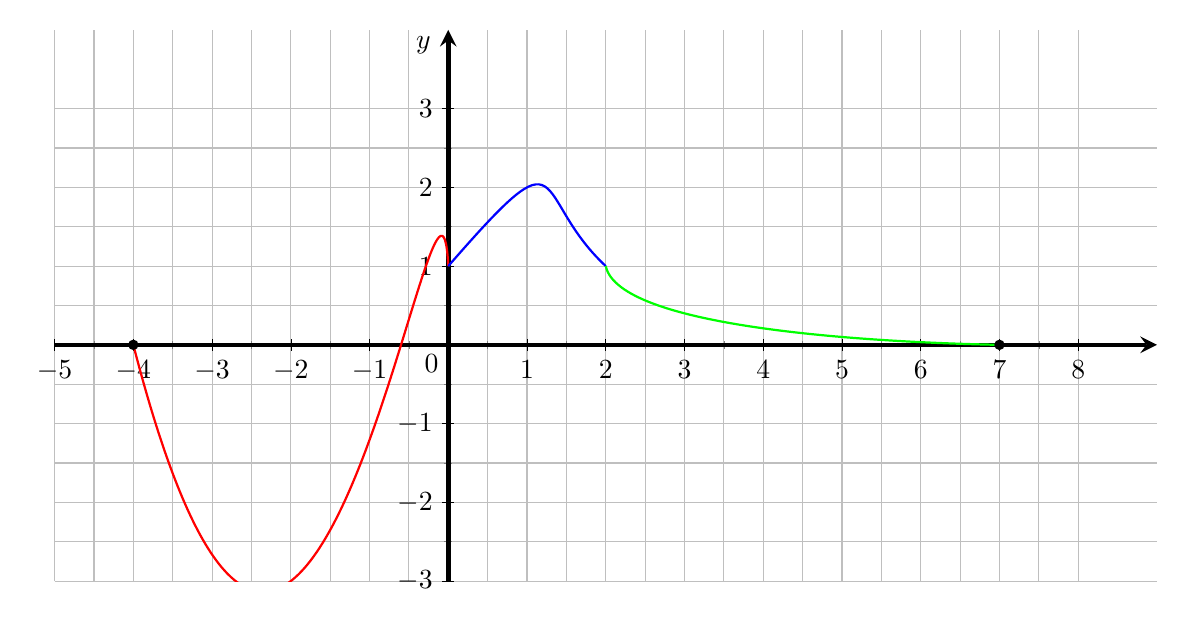
\begin{tikzpicture}

 \begin{axis}[
 restrict x to domain=-5:9, xmax=9, xmin=-5,
 restrict y to domain=-3:4, ymax=4, ymin=-3,
 x=1cm,
 y=1cm,
 axis x line = middle,
 axis y line = middle,
 axis line style =ultra thick,
 major tick style=black,
 grid=both,
 major grid style=lightgray,
 minor grid style=lightgray,
 minor tick num=1,
 xtick={-5,...,8},
 ytick={-3,...,3},
 samples=1000,
 >=stealth,
 ]

\addplot[
patch,
red,
patch type=cubic spline,
thick,
]
coordinates{
(-4,0) (0,1)(-2,-3) (-0.6,0) 
};

\addplot[
patch,
blue,
patch type=cubic spline,
thick,
]
coordinates{
(0,1) (2,1)(1,2)(1.4,1.8)
};

\addplot[
patch,
green,
patch type=cubic spline,
thick,
]
coordinates{
(2,1) (7,0)(3,0.4)(5,0.1)
};

\node[fill=black,circle,scale=0.4] at (-4,0){};
\node[fill=black,circle,scale=0.4] at (7,0){};

\node[below left] at (axis cs:0,0) {$0$};
\node[below] at (axis cs:9.8,-0.1) {$x$};
\node[left] at (axis cs:-0.1,3.8) {$y$};

\end{axis}
\end{tikzpicture}
\end{document}
